\documentclass[10pt,a4paper,oneside]{scrartcl}
\usepackage[latin1]{inputenc}
\usepackage{amsmath}
\usepackage{amsfonts}
\usepackage{amssymb}
\usepackage{makeidx}
\usepackage{graphicx}
\usepackage{booktabs}
\usepackage{tikz}
\usepackage[
	   style=ieee
	   ]
	   {biblatex}
\usepackage{mathtools}
\usepackage{enumitem}
\author{}
\title{Trie}
\date{}
\addbibresource{~/modules/References.bib}
\begin{document}
\maketitle
\paragraph{Notation}: \texttt{trie}
\paragraph{Description}: A structure for organizing sequential data hierarchically. Members of a previous generation can spawn infinitely many members of the next generation, but the data cannot be read out of sequence. In other words a parent can spawn any number of children, but cannot skip a generation. This ensures that all the data in a trie are related to each other properly. 

A simple kind of trie that everyone has used is a list: \\

\centering
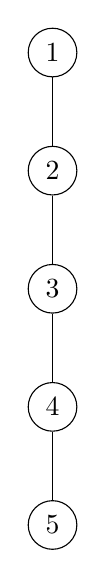
\begin{tikzpicture}[sibling distance=10em,
  every node/.style = {shape=circle,
    draw, align=center,
    top color=white, bottom color=blue!0}]]
  \node {1}
      child { node {2}
	child { node {3}
	  child { node {4}
	    child { node {5} } } } };
\end{tikzpicture}
\section{Trie Terminology\cite{wiki:xxx}}
	\begin{enumerate}[label=\textbf{\alph*})]
	\item [Root]--  The top (first) node in a tree.
	\item	[Child]--  A node directly connected to another node when moving away from the Root.
	\item	[Parent]--  The converse notion of a child.
	\item	[Siblings]--  A group of nodes with the same parent.
	\item	[Descendant]--  A node reachable by repeated proceeding from parent to child.
	\item	[Ancestor]--  A node reachable by repeated proceeding from child to parent.
	\item	[Leaf]\footnote{a.k.a. External Node}--  A node with no children.
	\item	[Branch\footnote{a.k.a. Internal Node}]--  A node with at least one child.
	\item	[Degree]--  The number of subtrees of a node.
	\item	[Edge]--  The connection between one node and another.
	\item	[Path]--  A sequence of nodes and edges connecting a node with a descendant.
	\item	[Level]--  The level of a node is defined by 1 + (the number of connections between the node and the root).
	\item	[Node Height]--  The height of a node is the number of edges on the longest path between that node and a leaf.
	\item	[Tree Height]--  The height of a tree is the height of its root node.
	\item	[Depth]--  The depth of a node is the number of edges from the tree's root node to the node.
	\item [Forest]-- A forest is a set of n $\geq  0$ disjoint trees.
	\end{enumerate}
\printbibliography
\end{document}

